\documentclass[11pt,a4paper]{article}
\usepackage[utf8]{inputenc}
\usepackage{amsmath}
\usepackage{amsfonts}
\usepackage{amssymb}

\usepackage{import}

\usepackage{graphicx}
\usepackage[colorlinks=true,citecolor=magenta,linkcolor=blue]{hyperref}

\usepackage[ruled,vlined]{algorithm2e}

\begin{document}

\begin{center}
\begin{Large}
\textbf{NIPoPoWs under Velvet Fork\\}
\end{Large}

\end{center}

\section{Introduction}
\import{sections/introduction}{intro.tex}

\section{Model Definition and Notation}

\section{NIPoPoWs under Soft or Hard Fork}
\import{sections/nipopows_hard_fork/}{nipopows_hard_fork.tex}

\section{NIPoPoWs under Velvet Fork}
\import{sections/nipopows_velvet_fork/}{nipopows_velvet_fork.tex}


\subsubsection{Security of Suffix Proofs}
\import{sections/nipopows_velvet_fork/}{suffix_security.tex}


\subsection{Infix Proofs}
The security of the original NIPoPoWs protocol suffers under velvet fork conditions for the case of infix proofs as well. Again, since blocks containing incorrect interlink pointers are accepted in the chain, the adversary may create an infix proof for a transaction included in a block mined on a different chain. This attack is presented in detail in the following.

An infix proof attack when applying the original protocol under a velvet fork should be obvious after our previous discussion. So consider the updated protocol for secure suffix proofs as described in the previous section. A problem here is that in the updated protocol some blocks are excluded from the interlink, while we should still be able to provide proofs for transactions included in any block of the chain. 

For this reason, let us initially consider an additional protocol patch suggesting to include a second interlink data structure in each block, which will be updated without any block exclusion, just as described in the original protocol and will be used for constructing infix proofs only. In order to be secure we could think of allowing using pointers of the second interlink only for the \textit{followDown} part of the algorithm. But still, the adversary may use an invalid pointer of a block visited during the \textit{followDown} procedure and jump to a block of another chain providing a transaction inclusion proof concerning that block. This attack is illustrated in Figure \ref{fig:infix_attack}.

\begin{figure}[h!]
	\begin{center}
		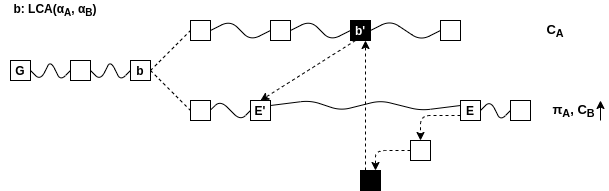
\includegraphics[scale=0.52]{figures/infix_attack.png}
	\end{center}
	\caption{\textit{Adversarial fork chain $C_A$ and an adversarial infix proof based on the chain adopted by an honest player. Wavy lines imply one or more blocks. Blocks generated by the adversary are colored black. Dashed arrows represent interlink pointers included in the proof as part of the \textit{followDown} procedure. The adversary provides infix proof for a transaction in block b'. }}
	\label{fig:infix_attack}
\end{figure}

Thus giving the ability to utilize invalid pointers even in a narrow block window can break the security of our protocol. 

\subsubsection*{Protocol patch for NIPoPoWs infix proofs under velvet fork}
However, since we have proved the security of suffix proofs we can include some more information in the blocks participating in these proofs in order to provide secure infix proofs as well.
 
Specifically, we suggest full nodes to maintain an authenticated data structure, let's say a Merkle Tree, for the blocks consisting the longest valid chain at each time point, and each block to additionally contain the Merkle Tree Root of  the blocks' Merkle Tree. In this way an infix proof will consist of a suffix proof in order to obtain the longest valid chain and a block inclusion proof for the block of interest. 

For example, in order to prove that a specific transaction $tx_1$ took place in a block $b'$, the Prover provides
\begin{itemize}
\item a suffix proof $\pi$
\item a block inclusion proof for $b'$, using the blocks' MTR existing in the tip of the suffix proof chain $\pi[-1]$
\item a transaction inclusion proof for $tx_1$ using the transactions' MTR of block $b'$
\end{itemize}

\subsubsection*{The velvet infix prover}
The construction of an infix proof is described in Algorithm \ref{alg:proveInfixVelvet}. In order to keep the algorithm generic enough for any infix-sensitive predicate, we provide the steps needed until the verification of the block of interest and consider the specific predicate answer as trivial to calculate given the block of interest. The infix prover accepts as input the full chain $C$ and a block of interest $b'$ and returns a proof consisting of the Merkle Tree proof of inclusion for $b'$ and a suffix proof.
\vspace{4mm}

\begin{algorithm}[H]
\SetAlgoNoLine
\DontPrintSemicolon
\SetKwProg{Fn}{function}{:}{\text{end function}}
\Fn{ProveInfixVelvet(C, b')}{
	$(\pi , \chi) \leftarrow Prove_{m,k}(C)$\;
	$tip = \pi [-1]$\;
	$\pi_{b'} \leftarrow \text{ConstrMTInclProof}(tip, b'.id )$\;
 
 
 	\Return ($\pi_b', (\pi, \chi)$)\;
}
 \caption{Velvet Infix Prover}
 \label{alg:proveInfixVelvet}
\end{algorithm}

\vspace{4mm}

\subsubsection*{The velvet infix verifier}
The infix proof verification algorithm is described in Algorithm \ref{alg:verifyInfixVelvet}.
Supposing that the verifier has already concluded to the longest valid chain $C$ after accepting and comparing constesting suffix proofs, the infix verification algorithm only has to confirm the Merkle-Tree inclusion proof for the block of interest $b'$.

\vspace{4mm}

\begin{algorithm}[H]
\SetAlgoNoLine
\DontPrintSemicolon
\SetKwProg{Fn}{function}{:}{\text{end function}}
\Fn{VerifyInfixVelvet($\pi_b', (\pi, \chi)$)}{
	$(\pi , \chi) \leftarrow Prove_{m,k}(C)$\;
	$tip = \pi [-1]$\;
	\Return $\text{VerMTInclProof}(tip.MTR_{blocks}, \pi_{b'}, b'.id )$\;
}
 \caption{Velvet Infix Verifier}
 \label{alg:verifyInfixVelvet}
\end{algorithm}

\vspace{4mm}

\bibliographystyle{plain} % We choose the "plain" reference style
\bibliography{refs} % Entries are in the "refs.bib" file

\end{document}